% Shared standalone design for the editable figure reconstructions.
\documentclass[tikz,border=5pt,10pt]{standalone}
\usepackage[T1]{fontenc}
\usepackage[utf8]{inputenc}
\usepackage{newpxtext,newpxmath}
\usepackage[scaled=.94]{sourcesanspro}
\usepackage{pgfplots}
\pgfplotsset{compat=1.18}
\usetikzlibrary{arrows.meta,calc,positioning,decorations.pathreplacing,
  decorations.markings,patterns,matrix,shapes.geometric,fit,backgrounds,
  intersections,angles,quotes}
\definecolor{ink}{HTML}{203746}
\definecolor{accent}{HTML}{146C78}
\definecolor{muted}{HTML}{667780}
\definecolor{signalred}{HTML}{B94B44}
\color{ink}
\tikzset{>=Latex,line width=.8pt,
  every node/.style={font=\small},
  axis/.style={->,draw=muted,line width=.5pt},
  guide/.style={draw=muted,dashed,line width=.45pt},
  curve/.style={draw=accent,line width=1pt},
  marker/.style={circle,fill=accent,inner sep=1.5pt},
  labelbox/.style={fill=white,inner sep=2pt}}

\begin{document}
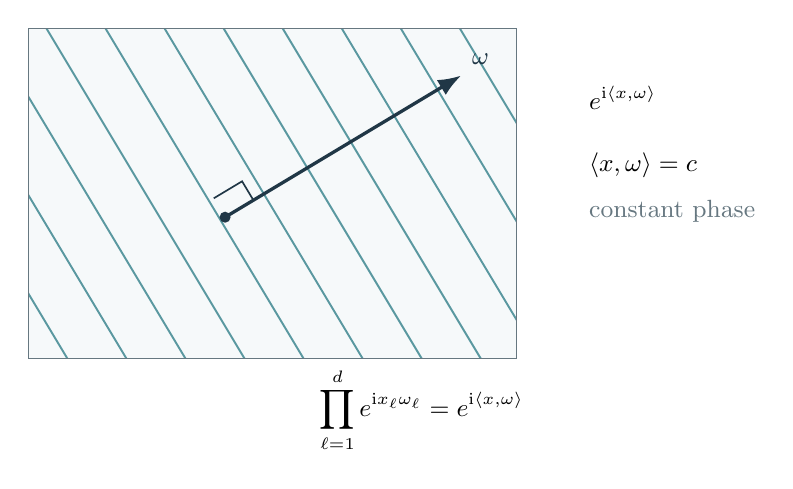
\begin{tikzpicture}[x=1cm,y=1cm]
\fill[accent!4] (0,0) rectangle(6.2,4.2);
\begin{scope}\clip (0,0) rectangle(6.2,4.2);
\foreach \a in {-1,-.25,...,9} {\draw[accent!70,line width=.7pt] (\a,0)--++(-2.52,4.2);}
\end{scope}
\draw[muted] (0,0) rectangle(6.2,4.2);
\fill[ink] (2.5,1.8) circle(2pt);
\draw[->,ink,line width=1.2pt] (2.5,1.8)--(5.5,3.6) node[above right] {$\omega$};
\draw[ink,line width=.6pt] (2.86,2.016)--(2.716,2.256)--(2.356,2.04);
\node[anchor=west,align=left] at (7,2.6) {$e^{\mathrm{i}\langle x,\omega\rangle}$\\[4mm]$\langle x,\omega\rangle=c$\\[2mm]\textcolor{muted}{constant phase}};
\node at (5,-.65) {$\displaystyle\prod_{\ell=1}^{d}e^{\mathrm{i}x_\ell\omega_\ell}=e^{\mathrm{i}\langle x,\omega\rangle}$};
\end{tikzpicture}
\end{document}
